\chapter{The Heteroscedastic Linear Mixed Model}
\label{chap:het_LMM}

% \cref{chap:dglm_human} described a statistical approach to QTL mapping that accounts for differential relatedness in the mapping population by including principle components of the genetic variation as regressors.
% This approach is heuristic, correcting for the large-scale relationships captured in the first handful of principle components, but not [finer] ones.
% Previous chapters dealt with differential relatedness obliquely, either assuming its absence or using a heuristic to correct for it, this chapter addresses it directly.

This chapter deals with the linear mixed model (LMM), a more elaborate statistical model for QTL mapping.
By estimating so called ``random effects'' with arbitrary covariance structure, the LMM can accommodate any pattern of differential relatedness in the mapping population.
The additional complexity of the LMM relative to the LM presents a computational challenge in applying it in large scale analyses, \eg on a dense set of genome wide markers.

This chapter proceeds as follows.
In section 1, we describe a verbose form of the LMM that emphasizes the meaning of each term in the model and describe how this model can be used to conduct a GWAS.
In section 2, we demonstrate a compact, but mathematically equivalent, form of the LMM that will be used for the remainder of the chapter.
In section 3, we illustrate how, given one parameter, $h^2$, the LMM can be fit by GLS.
In section 4, we illustrate how, given another parameter, $\bM$, the GLS problem can be simplified to the OLS problem, though we do not describe how to calculate $\bM$.
In section 5, we describe how these simplifications can be used to rapidly fit the LMM genomewide.
In section 6, we summarize a previously published result that demonstrates how to calculate $\bM$ for phenotypes with homoskedastic environmental residuals.
In section 7, we demonstrate a novel way to calculate $\bM$, that is valid whether the environmental residuals are homoskedastic or not.
In section 8, we show, through simulation, that for phenotypes with heteroscedastic environmental residuals, the novel value of $\bM$ leads to a more powerful test and better controls false positive rate.

% two mathematical tricks that allow for efficient 
% The rest of this chapter deals with algebraic tricks that allow efficient use of the LMM in the context of a GWAS.
% When a single parameter ($h^2$) is known, the LMM can be fit with the well-known generalized least squares (GLS) procedure.
% But even this procedure is too slow for use in GWAS.
% When two parameters are known ($h^2$ and $\bM$), the LMM can be fit by ordinary least squares (OLS), an extremely fast procedure appropriate for GWAS.


% Thus, 

% The simplicity offered in estimating all other parameters, given $h^2$ suggests a profile likelihood approach, but there are big matrix inversions required to fit even the LM, and given the many loci to be evaluated (each one defines a new LMM and thus a new LM), this approach is not immediatley tractable for GWAS.

% I describe a mathematical trick published in 2008 that allows for fitting the LM many times with only the work of the SLM when the environmental residuals are homoscedastic \citep{Kang2008}.
% Next, I describe a mathematical trick for the same that is valid whether the the environmental residuals are homoscedastic or not.
% Finally, I show simulation results that illustrate the benefit of accommodating heteroscedastic environmental residuals and demonstrate software I've developed that implements this procedure.

\section{The Linear Mixed Model}
The LMM models an observed phenotype, $\by$, as,
\begin{align}
	\by	&= \mathbf{1}\mu + \bX\bbeta + \bG\balpha + \ba + \be  \label{eq:lmm}
\end{align}

where $\mathbf{1}$ is a column vector of ones, $\bX$ is the design matrix of covariates, $\bG$ is the design matrix describing the genetic locus to be tested, and $\mu$, $\bbeta$, and $\balpha$ are unconstrained parameters that can be referred to as the population mean, the effect(s) of the covariate(s), and the effect(s) of the genetic factor(s) to be tested, respectively.
$\ba$ and $\be$ are so-called ``random effects'', estimated in the process of model fitting, but with constraints.
Specifically, they are modeled hierarchically as
\begin{align}
    \ba &\sim \N(0, \bK \tau^2) ,   \label{eq:a}\\
    \be &\sim \N(0, \bD \sigma^2)   \label{eq:e}
\end{align}
where $\bK$ is a known, positive semi-definite genomic similarity matrix, and $\bD$ is a known, diagonal residual variance matrix.
The scale parameters, $\tau^2$ and $\sigma^2$, are constrained only to be non-negative.

In the context of QTL mapping, the LMM is fit to each putative QTL, using $\bG$ to encode the locus design matrix and testing whether $\balpha = \bm{0}$.
If $\balpha \neq \bm{0}$, the locus is a QTL.
Here, we use the likelihood ratio test (LRT) to test how likely the observed difference between $\widehat{\balpha}$ and $\bm{0}$ is, due to chance alone.

In this context, the LRT requires ``fitting'' both a null and alternative version of the LMM, where the term ``fitting'' is shorthand for calculating the maximum likelihood value of all parameters.
The relevant alternative model is written in \cref{eq:lmm} and the relevant null model is identical except it excludes the term $\bG\balpha$.

% Two statistical tests used to determine whether $\balpha = \bm{0}$, the $t$ test and the likelihood ratio test (LRT), require computation of the values of the parameters that maximize the likelihood of the data.
\citet{Henderson1984} described a suite of procedures for fitting the LMM in a variety of situations, but Henderson's methods are of limited use in QTL mapping because they are computationally slow.
His focus was on estimation of breeding values ($\ba$ in \cref{eq:lmm}) and therefore the model only needed to be fit once, to one design matrix, and therefore speed was not a primary concern.
% Therefore, Henderson's methods are not of great use in the context of QTL mapping, where each putative QTL demands its own maximum likelihood model fit.

% In the context of QTL mapping, where $\bG$ encodes a single genetic locus, the model must be fit $L$ times, where $L$ is the number of loci to be tested, once for each locus.



% many different values of $\bX$... and compare to one with no genetic in $\bX$ to do LRT.
% The default way to do so would be to use Henderson's method each time, but this is very slow.
% A recent development described a matrix math trick to make this process fast when $\bD = \bI$.
% I first summarize that trick and then go on to describe a further trick that allows for fast fitting for any diagonal $\bD$.


% [define animal model, y, K, Z, D, two variance components]
% [all diagonal elements of K are 1, off diags can be also]




\section{Compact Specification of the LMM}

The LMM as specified in \cref{eq:lmm} is equivalent to:
\begin{align}
    \by &\sim \N(\bX_c\bbeta_c, \bV\lambda)
\end{align}
where fixed effects design matrices are combined into $\bX_c$ and the variance-covariance matrices of the random effects are combined into $\bV\lambda$.
Specifically, the covariate matrices and their effect vectors are compacted as
\begin{align}
    \bX_c      &= \left[1 \enspace \bX \enspace \bG \right]\\
    \bbeta_c   &= \left[\mu \enspace \bbeta\T \balpha\T \right]\T
\end{align}
Going forward, only the compact notation is used, so $\bX_c$ and $\bbeta_c$ will be referred to simply as $\bX$ and $\bbeta$.
The covariance matrices is compacted by use the re-parametrization,
\begin{align}
  h^2 &= \frac{\tau^2}{\tau^2 + \sigma^2}\\
  \lambda &= \tau^2 + \sigma^2
  % \bSigma &= \left(\bK \frac{\tau^2}{\tau^2 + \sigma^2} + \bD \frac{\sigma^2}{\tau^2 + \sigma^2}\right) (\tau^2 + \sigma^2)\\
      % &= \left( \bK h^2 + \bD (1 - h^2) \right) \lambda
\end{align}
and ``hiding'' the $h^2$ parameter inside the definition of $\bV$, which will be mathematically useful.
After defining 
\begin{align}
\bV &= \bK h^2 + \bD(1-h^2)
\shortintertext{we have}
\bK \tau^2 + \bD \sigma^2 &= \left(\bK h^2 + \bD(1-h^2)\right) \lambda\\
                            &= \bV \lambda \label{eq:lmm_covar}
\end{align}
% This parametrization implicitly uses the well-known narrow-sense heritability.
% The compaction of the variance-covariance term was accomplished by the reparametrization,
% based on the reparametrization:

This parameterization's usage of the narrow-sense heritability, $h^2$, has two benefits.
First, it is directly interpretable to geneticists.
And second, it is bounded to the range $[0, 1]$, which can be useful in a grid-based or gradient-based search for an optimal parameter value.


% \section{Strategy for Fitting the LMM Efficiently}

% \begin{align}
%   \argmin_b  
% \end{align}

% \begin{algorithm}
%   \SetKwInOut{Input}{Input}
%   \SetKwInOut{Output}{Output}
%   \Input{$\by$, $\bX$, $\bK$, and $\bD$}
%   \Output{For each column $l$ of $\bX$,  $\ell_{\text{ML}}(\by, \bX_l, \bK, \bD)$}
%   $(\bLK, \bUK) \gets \text{eigen decompose } \bK$\\
%   \For{$l \gets 1 \ldots L$} {
%     $\bM \gets \text{calculate } \bM$\\
%     $h^2 \gets \argmin_\ell$
%   }
%   \caption{GWAS Algorithm}
% \end{algorithm}




\section{Given \texorpdfstring{$h^2$}{h-squared}, the LMM problem reduces to the GLS problem}

Using the compact specification of the LMM, it is clear that for any given value of $h^2$, the LMM can be fit using generalized least squares (GLS).
\begin{align}
  \by \sim \N(\bX\bbeta, \bV \lambda)     \label{eq:gls}
\end{align}

The well-known ML estimates for $\bbeta$ and $\lambda$ are
\begin{align}
  \widehat{\bbeta}    &= (\bX \T \bV \inv \bX) \inv \bX \T \bV \inv \by\\
  \widehat{\lambda}   &= \norm{(\bX\widehat{\bbeta} - \by)\T(\bX\widehat{\bbeta} - \by)}{2}
\end{align}
but calculating them for many different values of $\bX$ is computationally demanding.
The most demanding step is the inversion of $(\bX \T \bV \inv \bX)$.
This procedure is not amenable to rapidly applying to many values of $\bX$ as will be necessary to conduct a GWAS.

We note here that the likelihood of \cref{eq:gls} is:
\begin{align}
    \ell(\bbeta, \lambda; \by, \bX, \bV) &= 
        -\frac{n}{2}\log(2\pi)
        -\frac{1}{2}\log|\bV\lambda|
        -           \frac{1}{2\lambda}
            (\by-\bX\bbeta)\T\bV\inv(\by-\bX\bbeta) \\
    &= 
        -\frac{n}{2}\log(2\pi)
        -\frac{1}{2}\log|\bV|
        -\frac{n}{2}\log\lambda
        - \frac{1}{2\lambda}
            (\by-\bX\bbeta)\T\bV\inv(\by-\bX\bbeta) \label{eq:lmm_loglik}
\end{align}
to which we will refer in the next section.
% which can be fit by GLS.
% And there is a known, closed-form, maximum likelihood estimator for its two parameters:

% In the context of a genome scan, we want to calculate these maximum likelihood estimators for a single phenotype, $\by$, genomic similarity, $\bK$ residual variance, $\bD$, and many different values of $\bX$ --- recall that the genetic variant(s) being investigated are in $\bG$.
% Also recall that, though we have described a parameterization that recapitulates a standard linear regression problem when $h^2$ is known, we do not, in general know the true value of $h^2$, so we will additionally want to optimize over all possible values of $h^2 \in [0, 1]$.

% We now describe a matrix algebra trick that allows us to increases the up-front computational cost of fitting the linear regression model \cref{eq:gls}, but drastically decreases the computational cost for each new value of $\bX$.


\section{Given \texorpdfstring{$\bM$}{M}, the GLS problem reduces to the OLS problem}
\label{sec:givenM}

Although the simplification of the LMM fitting process to the GLS procedure did not immediately result in a profound increase in computational efficiency, it will prove amenable to further simplification.
Take as given a matrix, $\bM$, that has the property
\begin{align}
	\bM \T \bM = \bV \inv
\end{align}
where $\bV$ is the covariance of $\by$, as defined in \cref{eq:lmm_covar}.
We can use $\bM$ to define a ``rotated'' phenotype vector, $\by_r = \bM \by$, which can be shown to have identity covariance.
\begin{align}
\var(\by_r) &= \var(\bM \by) \\
            &= \bM \var(\by) \bM \T\\
            &= \bM \bV \bM \T \\
            &= \bI
\end{align}
The last step can be verified by:
\begin{align}
  \bM \bV \bM \T            &= \bI\\
  \bM \T \bM \bV \bM \T \bM &= \bM \T \bM \\
  \bV \inv \bV \bV \inv     &= \bV \inv\\
  \bV \inv                  &= \bV \inv
\end{align}

Because $\by_r$ has identity covariance, it can be modeled with a linear model of the form:
\begin{align}
    \by_r &\sim \N(\bX_r \bbeta_r, \, \bI \lambda_r) \label{eq:ols}
\end{align}
where $\bX_r = \bM \bX$ is a ``rotated'' covariate matrix.
This linear model can be solved by ordinary least squares (OLS), which is computationally efficient and numerically stable when solved by the QR decomposition.
The well-known ML estimates of $\bbeta_r$ and $\lambda_r$ are
\begin{align}
    \widehat{\bbeta_r}    &= (\bX_r \T \bX_r) \inv \bX_r \T \by_r\\
    \widehat{\lambda_r}   &= \norm{(\bX_r \widehat{\bbeta_r} - \by_r)\T(\bX_r \widehat{\bbeta_r} - \by_r)}{2}
\end{align}

It can be shown that $\widehat{\bbeta_r} = \widehat{\bbeta}$ and $\widehat{\lambda_r} = \widehat{\lambda}$.

\begin{align}
  \widehat{\bbeta_r}    &= (\bX_r \T \bX_r) \inv \bX_r \T \by_r\\
                        &= ((\bM \bX)\T (\bM \bX)) \inv (\bM \bX)\T \bM \by\\
                        &= (\bX\T \bM\T \bM \bX))\inv \bX\T \bM\T \bM \by\\
                        &= (\bX\T \bV\inv \bX)\inv \bX\T \bV\inv \by\\
                        &= \widehat{\bbeta}
\end{align}

The OLS problem (\cref{eq:ols}) has log likelihood:
\begin{align}
    \ell(\bbeta_r, \lambda_r; \bX_r, \by_r) 
    &=    -\frac{n}{2}\log(2\pi)
          -\frac{1}{2}\log|\bI|
          -\frac{n}{2}\log\lambda_r
          -\frac{1}{2\lambda_r}
          (\by_r - \bX_r)\T (\by_r - \bX_r\bbeta_r)\\
    & =
          -\frac{n}{2}\log(2\pi)
          -\frac{n}{2}\log\lambda_r
          -\frac{1}{2\lambda_r}
          (\bM\by - \bM\bX\bbeta_r)\T (\bM\by - \bM\bX\bbeta_r)\\
    &=    -\frac{n}{2}\log(2\pi)
          -\frac{n}{2}\log\lambda_r
          -\frac{1}{2\lambda_r}
          (\by - \bX\bbeta_r)\T \bM\T \bM (\by - \bX\bbeta_r)\\
    &=    -\frac{n}{2}\log(2\pi)
          -\frac{n}{2}\log\lambda_r
          -\frac{1}{2\lambda_r}
          (\by-\bX\bbeta_r)\T \bV\inv (\by-\bX\bbeta_r)
\end{align}

Note that the likelihood of the OLS problem (\cref{eq:ols}) differs from that of the GLS problem by only a constant, $\frac{1}{2}\log|\bV|$.
\begin{align}
  \ell(\bbeta_r, \lambda_r; \bX_r, \by_r) = \ell(\bbeta, \lambda; \bX, \by) -\frac{1}{2}\log|\bV|
\end{align}
thus, for fixed $h^2$ (and thus fixed $\bV$), these likelihoods reach their maxima at the same location in parameter space and thus
\begin{align}
\widehat{\bbeta_r} &= \widehat{\bbeta}\\
\widehat{\lambda_r} & = \widehat{\lambda}
\end{align}

This identity makes possible a strategy to use the LMM to conduct a GWAS.
Specifically, by using Brent's method to optimize over $h^2$, and therefore using a fixed $h^2$ at each step, and using $\bM$ to fit the model by OLS rather than GLS at each step, the LMM can be rapidly fit to any $\bX$.
But this procedure requires the ability to rapidly calculate $\bM$ and $\log \left| \bM \right|$, which we have thus far not addressed.
In the following sections we address the calculation of $\bM$.

% This observation makes possible the following procedure for fitting the LMM to many genetic loci:
% For a grid of values of $h^2$, calculate $\bV$ and $\log|\bV|$.



% Because $\by$ has identifiy covariance, the ML values of $\bbeta_r$ and $\lambda_r$ can be computed rapidly by ordinary least squares (OLS).
% These estimates are
% The former is typically computed with the QR decomposition method.
% Thus we have established that, given $\by$ and $\bM$, we can rapidly compute the ML values of $\beta$ and $\lambda$.


\section{\texorpdfstring{$\bM$}{M} for the Homoscedastic LMM}

\citet{Kang2008} proposed the strategy for GWAS described above and proposed a value of $\bM$ that is computationally efficient and is valid when $\bD = \bI$.
This advance was termed ``EMMA'', an acronym for efficient mixed-model analysis.
Their approach used a slightly different, but mathematically equivalent, parameterization of the variance components, but we convert it into the $h^2, \lambda$ parameterization here for consistency with the rest of this chapter.
The differences in parameterization do not change the likelihood of the model and do not influence any results.
% and analytical derivatives of the likelihood with respect to...
% [but used a slightly different parameterization]

\subsection{Kang's \texorpdfstring{$\bM$}{M}}

\begin{align}
  \bM_\text{hom} &= \left( h^2\bLK + (1-h^2)\bI \right)\neghalfpow \bUK \T
\end{align}
where $\bLK$ and $\bUK$ are the eigenvalue matrix and eigenvector matrix of $\bK$, respectively.

\subsection{Validity}
It can be verified that $\bM_\text{hom} \T \bM_\text{hom} = \bV\inv$.
First, compute a useful form of $\bV$ and $\bV\inv$.

\begin{align}
  \bV &= h^2\bK + (1-h^2)\bI     \tageq{definition}\\
      &= h^2 \bUK \bLK \bUK\T + (1-h^2)\bI \tageq{eigen decomposition}\\
      &= h^2 \bUK \bLK \bUK\T + (1-h^2)\bUK \bUK\T \tageq{eigen vectors of real symmetric are orthonormal}\\
      &= \bUK \left(h^2 \bLK + (1 - h^2) \bI \right) \bUK\T \tageq{distributive property}
\shortintertext{and thus,}
\bV\inv &= \bUK \left(h^2 \bLK + (1 - h^2) \bI \right)\inv \bUK\T \tageq{inverse by eigen decomposition}
\end{align}

Then, we can verify the necessary equality.
\begin{align}
  \bM \T \bM  &= \left(\left(h^2\bLK + (1-h^2)\bI\right)\neghalfpow \bUK \T \right)\T \left(\left(h^2\bLK + (1-h^2)\bI\right)\neghalfpow \bUK \T\right) \tageq{definition} \\
              &= \bUK \left(h^2\bLK + (1-h^2)\bI\right)\neghalfpow \left(h^2\bLK + (1-h^2)\bI\right)\neghalfpow \bUK \T  \tageq{transpose of product}\\
              &= \bUK \left(h^2\bLK + (1-h^2)\bI\right)\inv \bUK \T \tageq{product of roots}\\
              &= \bV\inv \tageq{from above}
\end{align}


\subsection{Calculation of \texorpdfstring{$\log \left| \bV \right|$}{log(det(V))}}

As described in \cref{sec:givenM}, $\log \left| \bV \right|$ is necessary to calculate the likelihood of the original model from the likelihood of the rotated model.
In the case of $\bM_\text{hom}$ it is straightforward to calculate.
The determinant of any matrix is equal to the product of its eigen values, so the log of the determinant is simply the sum of its eigen values.

\begin{align}
  \log \left| \bV \right| = \sum_{i=1}^n{h^2 \lambda_Ki + (1 - h^2)}
\end{align}


\section{\texorpdfstring{$\bM$}{M} for the Heteroscedastic LMM}

The above $\bM$ is valid only when $\bD = \bI$ because the transition from Equation 5.43 to 5.44 in the validity proof required that the product of $\bUK \bI \bUK\T$ be a diagonal matrix.
If $\bI$ were replaced by any other diagonal matrix, this product would not be diagonal.

In the more general situation, where the phenotype associated with some genotypes is known with more certainty than the phenotype associated with other genotypes, it would be preferable to use a covariance matrix for the residual variance that reflects this reality.
Here, I propose a multiplier matrix that yields all the speed up of the above trick, but remains valid for any diagonal residual covariance matrix.

\subsection{Proposal}

\begin{align}
	\bM &= (\bLL + \delta \bI)^{-\frac{1}{2}}\bUL\T \bD^{-\frac{1}{2}}\\
\shortintertext{where}
	\bL &= \bD^{-\frac{1}{2}}\bK \bD^{-\frac{1}{2}}\\
\shortintertext{and}
	\bL &= \bUL \bLL \bUL^T
\end{align}
is its eigen decomposition


\subsection{Validity}

To be a valid multiplier matrix, $\bM$ must have the property:
\begin{equation}
  \bM \T \bM = \bV\inv
\end{equation}
	


% I verify this by showing that
% \[
% 	\bV \bM\T \bM = \bM\T \bM \bV = \bI
% \]

% I verify by direct calculation:



\begin{proof}
First, derive a useful form of $\bV$.
\begin{align}
\bV &= \bK + \delta \bD                                                                                             \tageq{definition}\\
    &= \bD\halfpow \bD\neghalfpow (\bK + \delta \bD)                                                                \tageq{pre-multiply by $\bD\halfpow \bD\neghalfpow = \bI$}\\
    &= \bD\halfpow \bD\neghalfpow (\bK + \delta \bD) \bD\neghalfpow \bD\halfpow 										                \tageq{post-multiply by $\bD\neghalfpow \bD\halfpow = \bI$}\\
    &= \bD\halfpow(\bD\neghalfpow \bK \bD\neghalfpow + \delta \bD\neghalfpow \bD \bD\neghalfpow)\bD\halfpow         \tageq{distribute $\bD\neghalfpow$ in}\\
    &= \bD\halfpow(\bD\neghalfpow \bK \bD\neghalfpow + \delta \bI) \bD\halfpow                                  		\tageq{definition of root inverse}\\
    &= \bD\halfpow(\bL + \delta \bI) \bD\halfpow                                                                 		\tageq{define: $\bL = \bD\neghalfpow\bK \bD\neghalfpow$}\\
    &= \bD\halfpow(\bUL \bLL \bUL \T + \delta \bI) \bD\halfpow                                                			\tageq{eigen decomposition of $\bL$}\\
    &= \bD\halfpow(\bUL \bLL \bUL \T + \delta \bUL \bUL \T)\bD\halfpow                                         			\tageq{property of eigen vectors}\\
    &= \bD\halfpow\bUL (\bLL + \delta \bI) \bUL \T \bD\halfpow                                                			\tageq{distributive property}
\end{align}
and invert it
\begin{align}
\bV\inv &= \left( \bD\halfpow\bUL (\bLL + \delta \bI) \bUL \T \bD\halfpow \right)\inv                                         \tageq{definition}\\
        &= \left( \bD\halfpow \right)\inv \left( \bUL (\bLL + \delta \bI) \bUL\T \right)\inv \left( \bD\halfpow \right)\inv   \tageq{inverse of product}\\
        &= \bD\neghalfpow \left( \bUL (\bLL + \delta \bI) \bUL\T \right)\inv \bD\neghalfpow                                   \tageq{inverse of diagonal matrix}\\
        &= \bD\neghalfpow \bUL (\bLL + \delta \bI)\inv \bUL\T  \bD\neghalfpow                                                 \tageq{inverse of eigen decomposition}
\end{align}
and compare to $\bM\T \bM$
\begin{align}
\bM \T \bM 	&= \left((\bLL + \delta \bI)\neghalfpow \bUL\T \bD\neghalfpow 	\right)\T   \left((\bLL + \delta \bI)\neghalfpow \bUL\T \bD\neghalfpow \right) \tageq{definition}\\
			&= \left(\bD\neghalfpow \bUL (\bLL + \delta \bI)\neghalfpow 	\right)  \left((\bLL + \delta \bI)\neghalfpow \bUL\T \bD\neghalfpow		\right)          \tageq{transpose of product}\\
			&= \bD\neghalfpow \bUL \left( (\bLL + \delta \bI)\neghalfpow 	(\bLL + \delta \bI)\neghalfpow \right)	\bUL\T \bD\neghalfpow                          \tageq{associative property}\\
			&= \bD\neghalfpow \bUL (\bLL + \delta \bI)\inv \bUL\T \bD\neghalfpow                                                                                 \tageq{definition of root inverse}
			% &= \bD\neghalfpow \left( \bUL (\bLL + \delta \bI) \bUL\T \right)\inv \bD\neghalfpow 																\tag*{inverse of eigen decomposition}\\
\end{align}
\end{proof}


\subsection{Calculation of \texorpdfstring{$\log \left| \bV \right|$}{log(det(V))}}

As with $\bM_\text{hom}$, the calculation of $\log \left| \bV \right|$ comes almost for free after calculating $\bM$.

\begin{align}
  \bV                     &= \bD\halfpow \left( h^2\bL + (1-h^2)\bI \right) \bD\halfpow\\
  \log \left| \bV \right| &= \log \left( \left| \bD\halfpow \left( h^2\bL + (1-h^2)\bI \right) \bD\halfpow \right| \right)\\
                          &= \log \left( \left| \bD\halfpow \right| \left| \left( h^2\bL + (1-h^2)\bI \right) \right| \left| \bD\halfpow \right| \right)\\
                          &= \log \left( \left| \bD \right| \left| \left( h^2\bL + (1-h^2)\bI \right) \right| \right)\\
                          &= \log \left( \left| \bD \right| \right) + \log \left(\left| \left( h^2\bL + (1-h^2)\bI \right) \right| \right)                          
                          % &= \log \left( \left| \bD \right| \right) + \log \left(\left| \left( h^2\bUL \bLL \bUL\T + (1-h^2)\bUL\bUL\T \right) \right| \right)\\
                          % &= \log \left( \left| \bD \right| \right) + \log \left(\left| \left( \bUL \left( h^2\bLL + (1-h^2)\bI \right) \bUL\T \right) \right| \right)\\
\end{align}

At this point, the problem is reduced to two terms.
The first is log of the determinant of a diagonal matrix, which is simply the sum of its elements.
The second is the log of the determinant of a covariance matrix expressed in the same form as was present in the homoskedastic setting, simply with $\bL$ in place of $\bK$ and can be solved in the same way.
Specifically,

\begin{align}
  \log \left( \left| \bD \right| \right) &= \sum_{i = 1}^n{d_i}
\shortintertext{and}
  \log \left(\left| \left( h^2\bL + (1-h^2)\bI \right) \right| \right) &= \sum_{i=1}^n{h^2 \lambda_Li + (1 - h^2)}
\end{align}

% Now we have
% \begin{align}
% \bM\T \bM 	&= 	\left( \bD\halfpow\bUL (\bLL + \delta \bI) \bUL \T \bD\halfpow 		\right)		
% 					\left((\bLL + \delta \bI)\neghalfpow \bUL\T \bD\neghalfpow 	\right)\T
% 					\left((\bLL + \delta \bI)\neghalfpow \bUL\T \bD\neghalfpow 	\right) 				\tag*{definitions}\\
% 				&= 	\left( \bD\halfpow\bUL (\bLL + \delta \bI) \bUL\T \bD\halfpow 		\right)
% 					\left(\bD\neghalfpow \bUL (\bLL + \delta \bI)\neghalfpow 	\right)
% 					\left((\bLL + \delta \bI)\neghalfpow \bUL\T \bD\neghalfpow 	\right)					\tag*{transpose of product}\\
% 				&= 	\bD\halfpow\bUL (\bLL + \delta \bI) \bUL\T \left(\bD\halfpow 		
% 					\bD\neghalfpow \right) \bUL \left((\bLL + \delta \bI)\neghalfpow
% 					(\bLL + \delta \bI)\neghalfpow \right) \bUL\T \bD\neghalfpow						\tag*{associative property of matrix multiplication}\\
% 				&= 	\bD\halfpow\bUL (\bLL + \delta \bI) \bUL\T
% 					 \bUL \left(\bLL + \delta \bI \right)\inv  \bUL\T \bD\neghalfpow					\tag*{definition of root and root inverse}\\
% 				&= 	\bD\halfpow\bUL (\bLL + \delta \bI) \left(\bLL + \delta \bI \right)\inv  \bUL\T \bD\neghalfpow					\tag*{property of eigenvector matrix}\\
% 				&= 	\bD\halfpow\bUL  \bUL\T \bD\neghalfpow					\tag*{definition of inverse}\\
% 				&= 	\bD\halfpow \bD\neghalfpow					\tag*{property of eigenvector matrix}\\
% 				&= \bI 													\tag*{definition of inverse}
% \end{align}

% 	&= [D^{\frac{1}{2}}U_L (\Lambda_L + \delta I) U_L^T D^{\frac{1}{2}}] [D^{-\frac{1}{2}}U_L(\Lambda_L+\delta I)^{-\frac{1}{2}}][(D^{-\frac{1}{2}}U_L(\Lambda_L+\delta I)^{-\frac{1}{2}})^T]\\
%     		&= D^{\frac{1}{2}}U_L (\Lambda_L + \delta I) U_L^T D^{\frac{1}{2}}D^{-\frac{1}{2}}U_L(\Lambda_L+\delta I)^{-\frac{1}{2}}(\Lambda_L+\delta I)^{-\frac{1}{2}T} U_L^T D^{-\frac{1}{2}T} \\
%     		&= D^{\frac{1}{2}}U_L (\Lambda_L + \delta I) U_L^T D^{\frac{1}{2}}D^{-\frac{1}{2}}U_L(\Lambda_L+\delta I)^{-1} U_L^T D^{-\frac{1}{2}T} \\
%     		&= D^{\frac{1}{2}}U_L (\Lambda_L + \delta I) U_L^T U_L(\Lambda_L+\delta I)^{-1} U_L^T D^{-\frac{1}{2}T} \\
%     		&= D^{\frac{1}{2}}U_L (\Lambda_L + \delta I) (\Lambda_L+\delta I)^{-1} U_L^T D^{-\frac{1}{2}T} \\
%     		&= D^{\frac{1}{2}}U_L U_L^T D^{-\frac{1}{2}T} \\
%     		&= D^{\frac{1}{2}} D^{-\frac{1}{2}T} \\
%     		&= I
% \end{align}

\newpage
\section{Simulation Results}

It is expected that, when the weights are known by oracle, the weighted LMM should outperform the unweighted LMM in two ways.
First, it should accurately control the FPR.
And second, it should better discriminate between real and spurious signals.


\subsection{FPR Control}

wISAM has better FPR control.  Explain the example in detail and then refer to some of the panels in the megafigs.

\begin{figure}
  \centering
  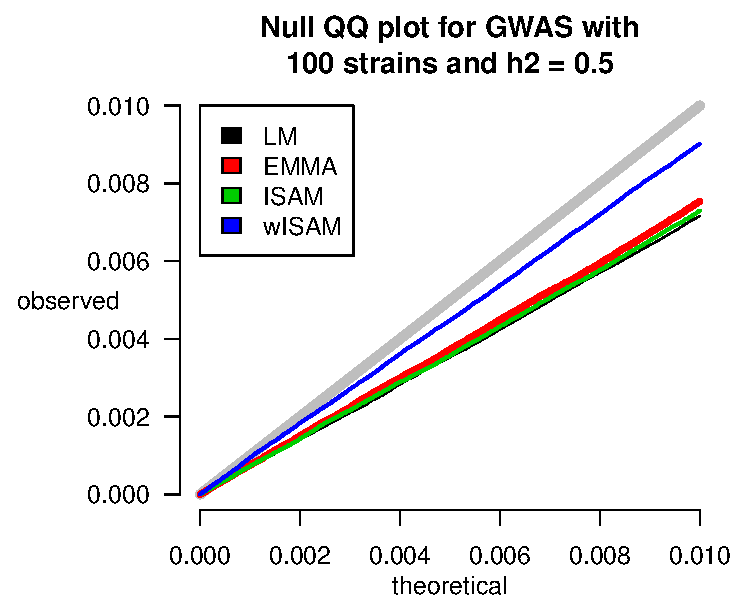
\includegraphics[width = 0.5\textwidth]{images/exampleQQ.pdf}
  \caption{explain this}
  \label{fig:exampleQQ}
\end{figure}

\begin{sidewaysfigure}
  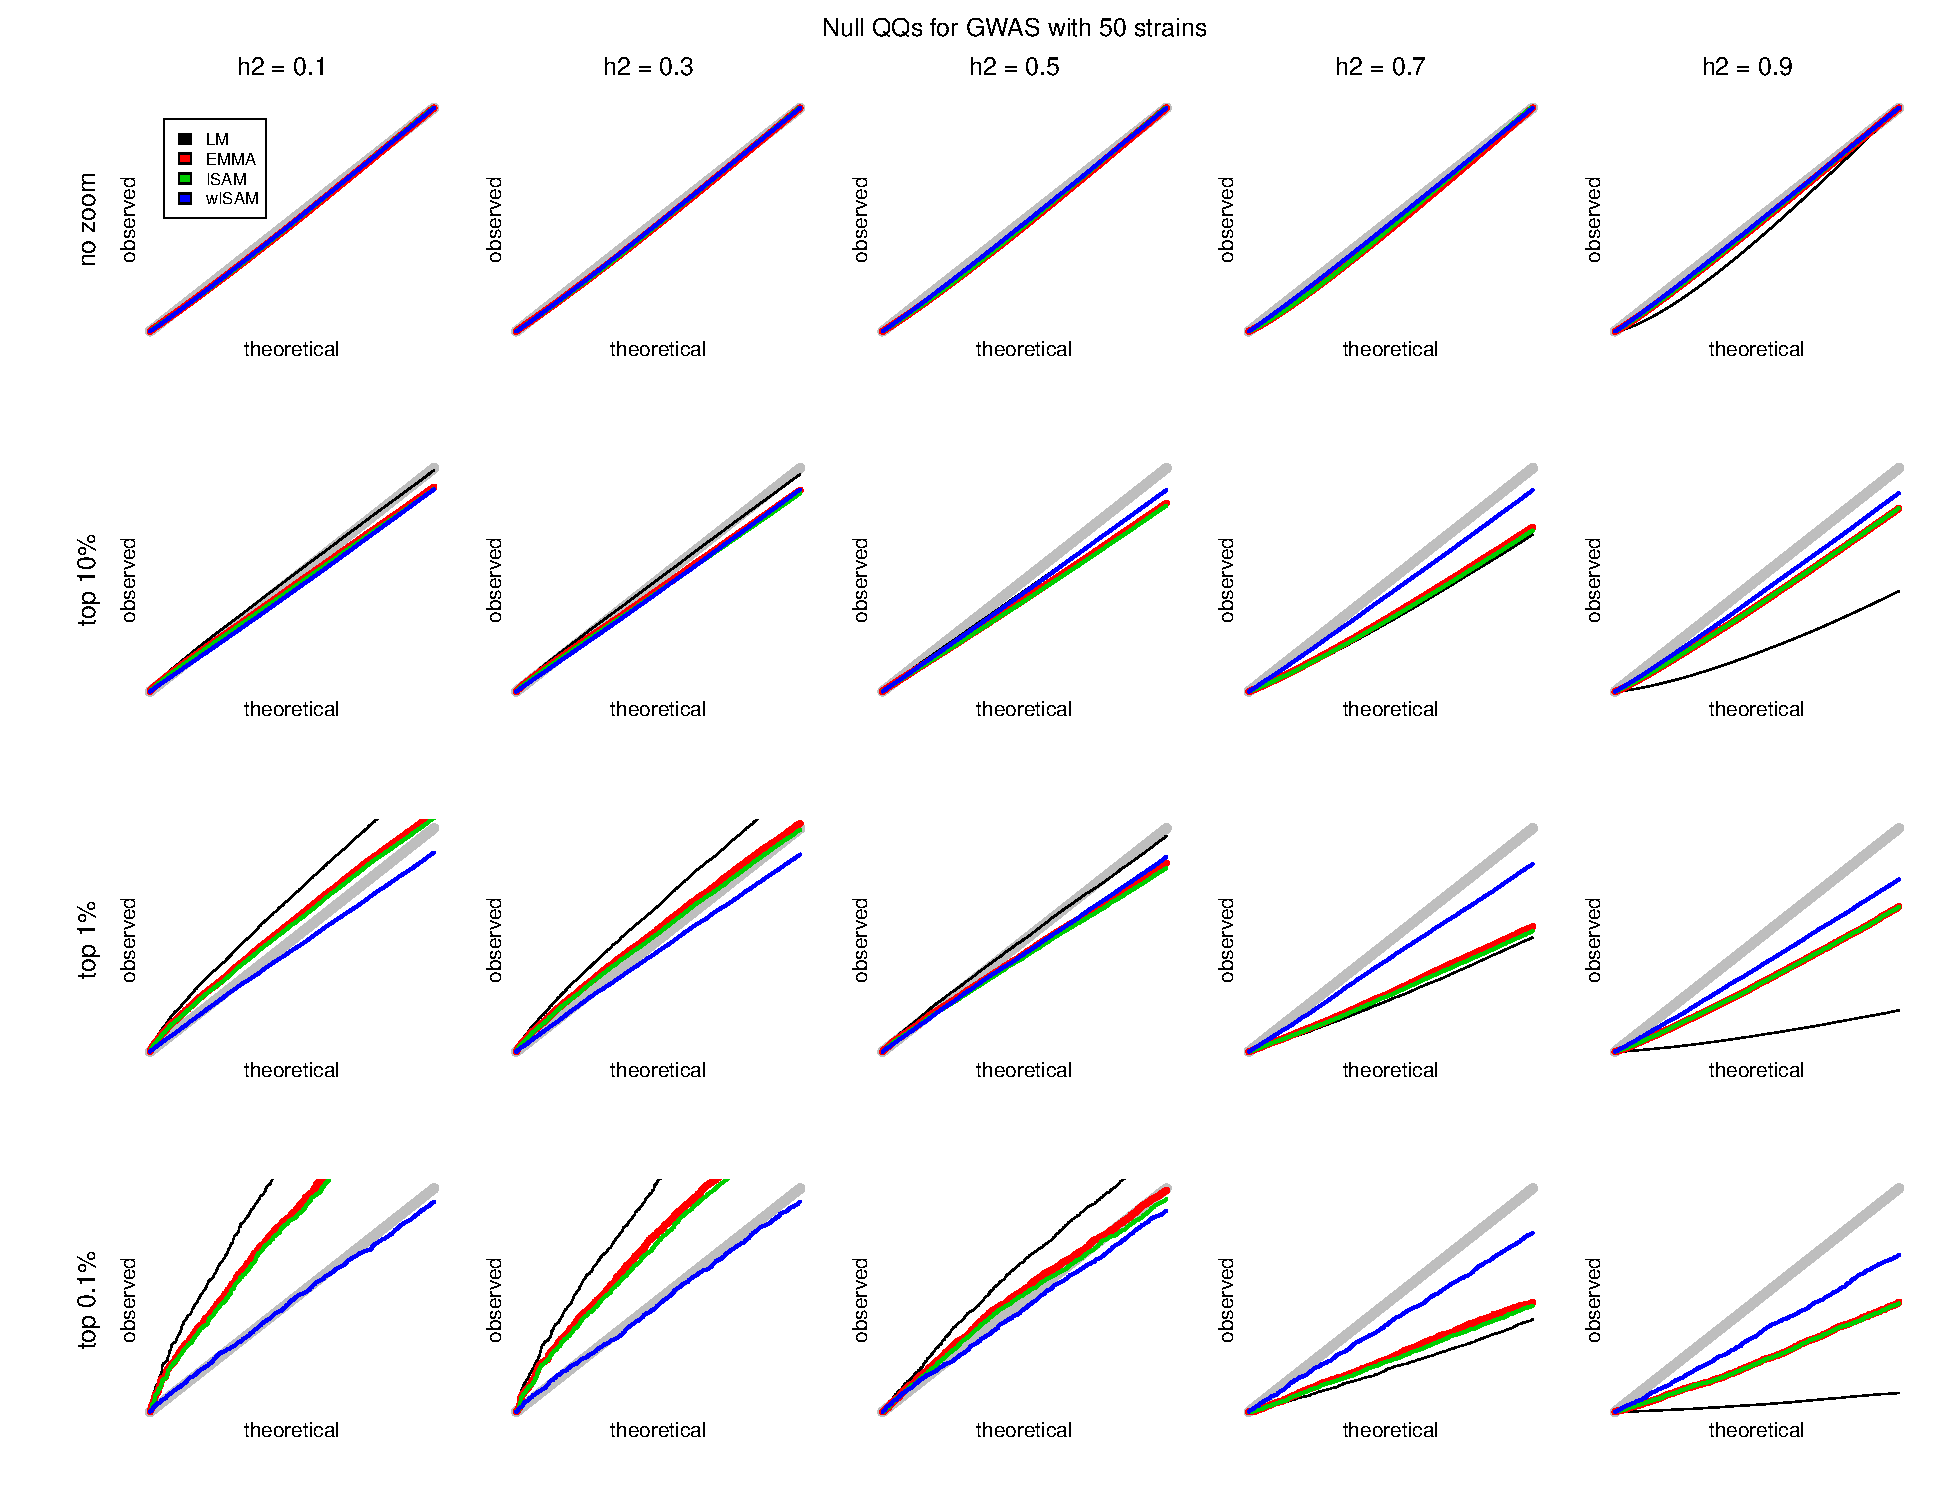
\includegraphics[width = \textwidth]{images/2018-05-19alt_heterosked_sims_nstrain=50_nsnps=100_nsims=10000.pdf}
\end{sidewaysfigure}

\begin{sidewaysfigure}
  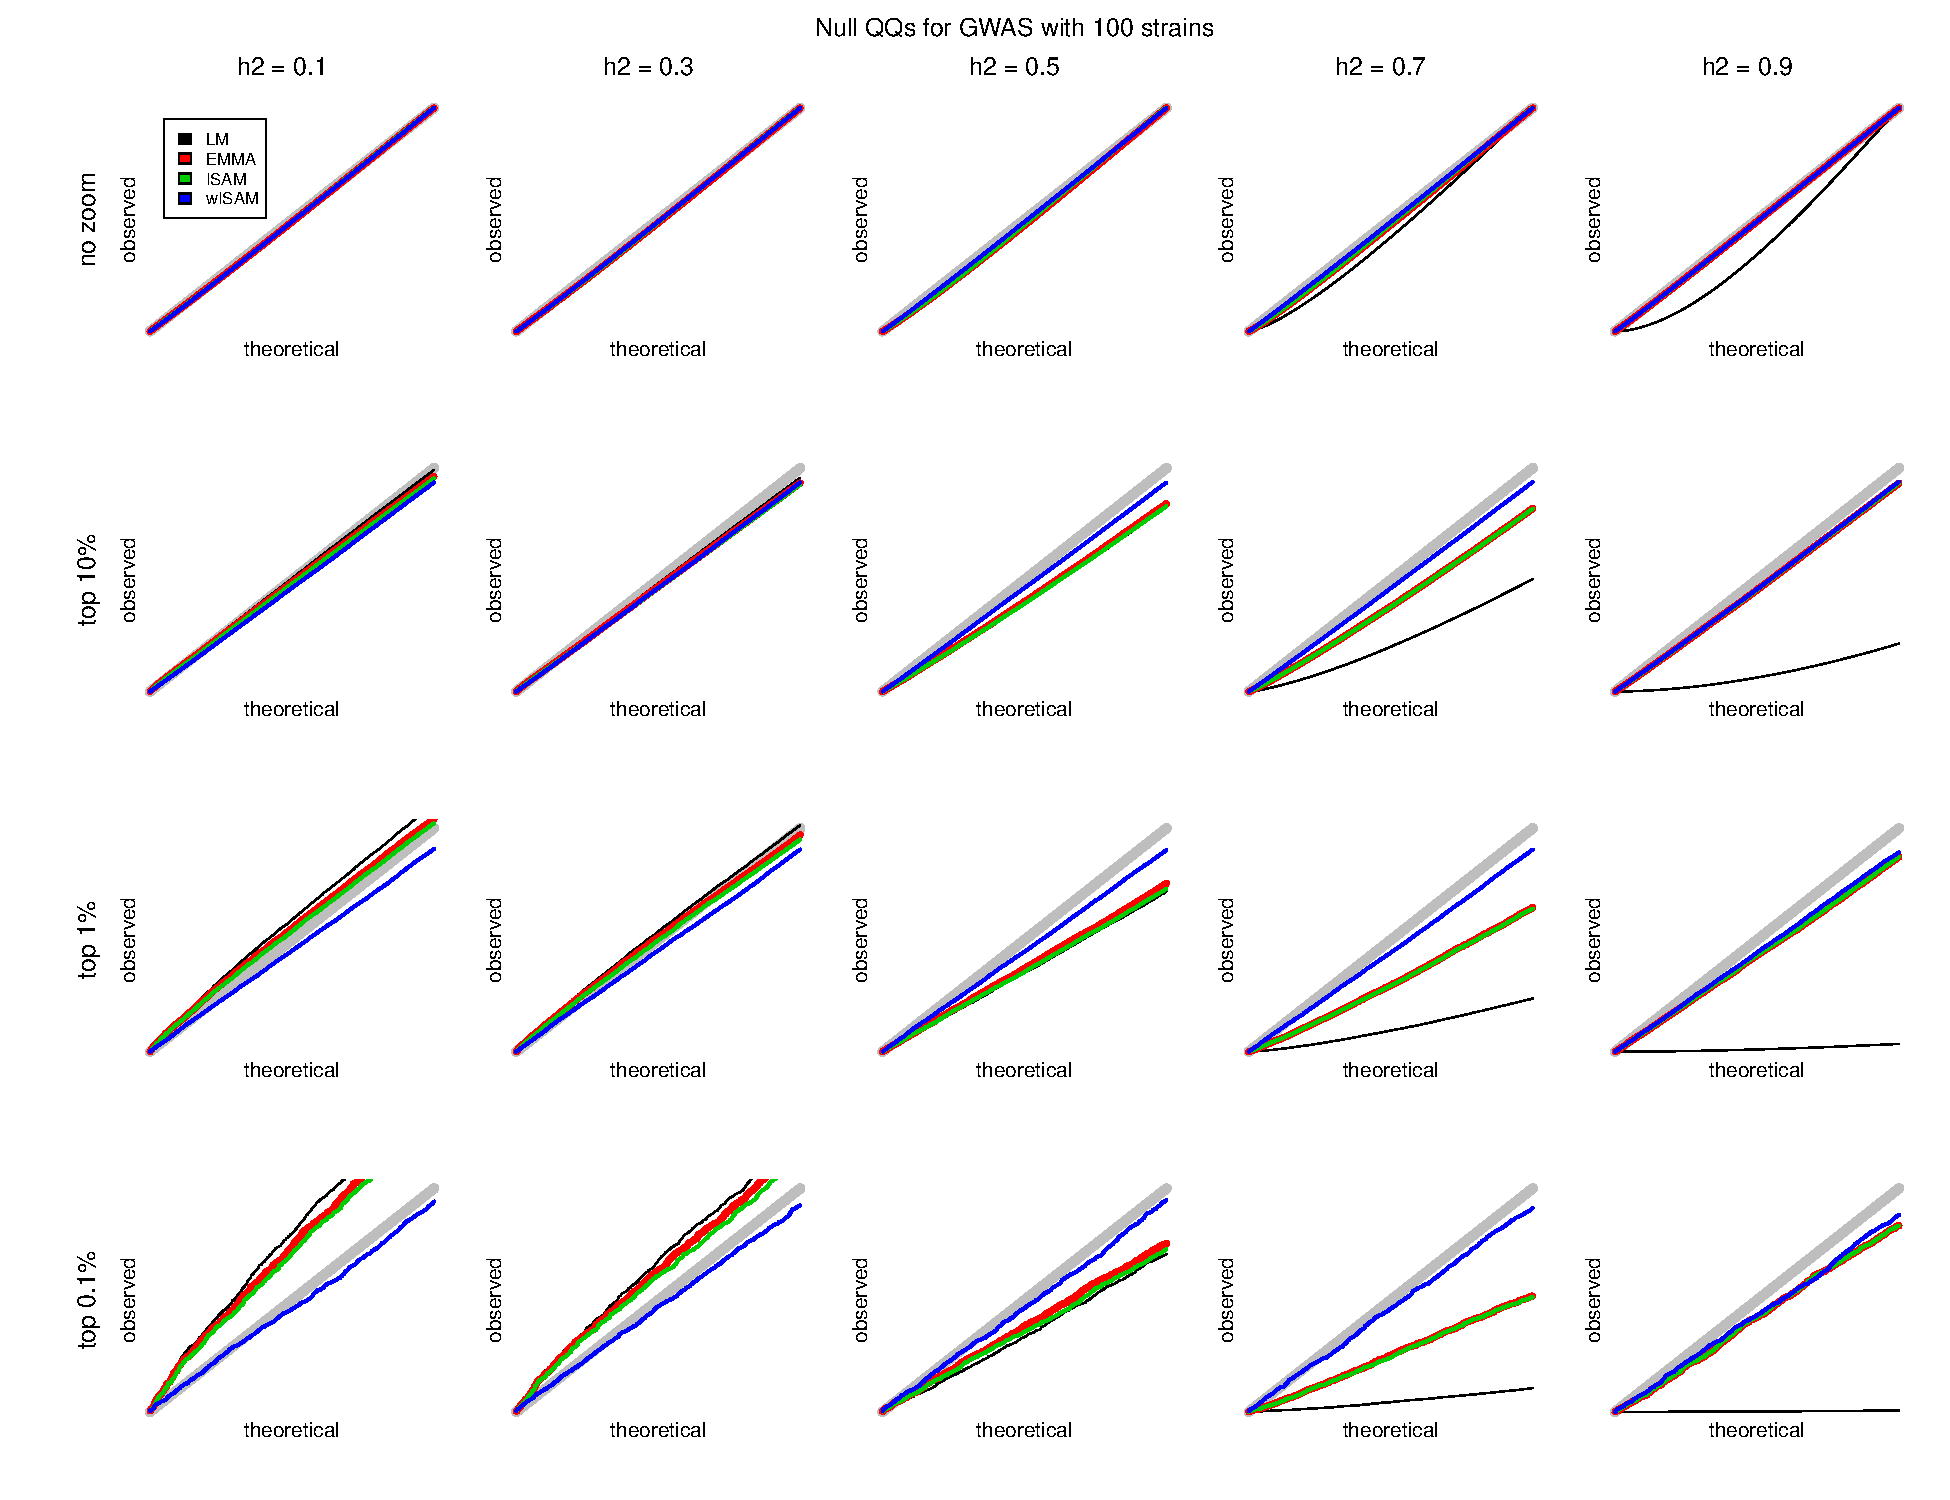
\includegraphics[width = \textwidth]{images/2018-05-19alt_heterosked_sims_nstrain=100_nsnps=100_nsims=10000.pdf}
\end{sidewaysfigure}

\begin{sidewaysfigure}
  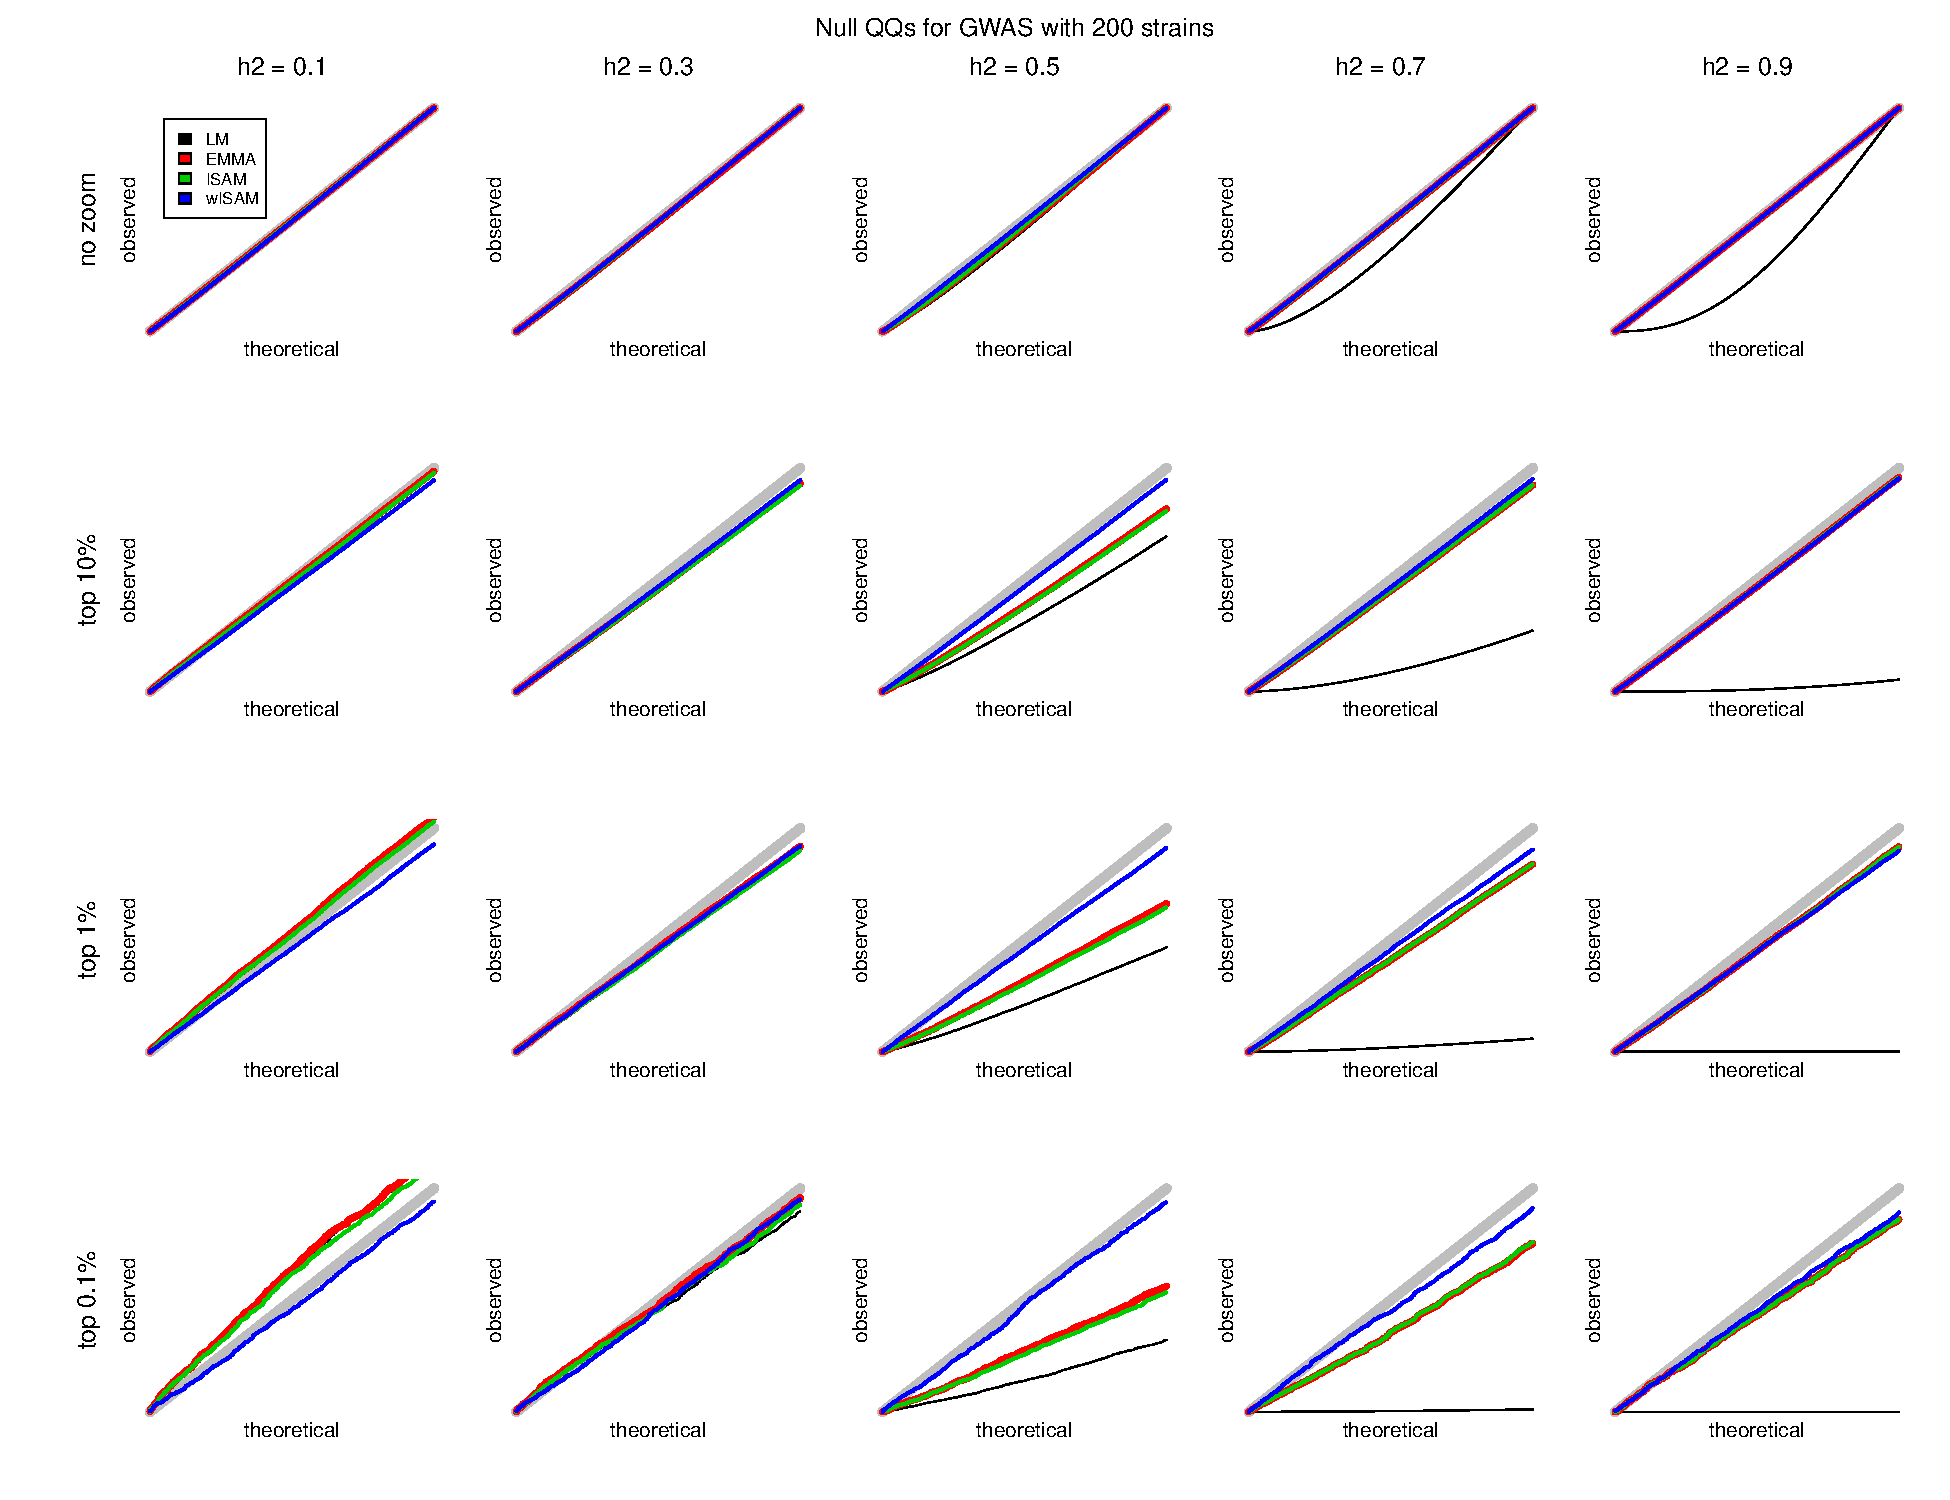
\includegraphics[width = \textwidth]{images/2018-05-19alt_heterosked_sims_nstrain=200_nsnps=100_nsims=10000.pdf}
\end{sidewaysfigure}


\subsection{Discrimination between real and spurious signals}

\begin{figure}
  \centering
  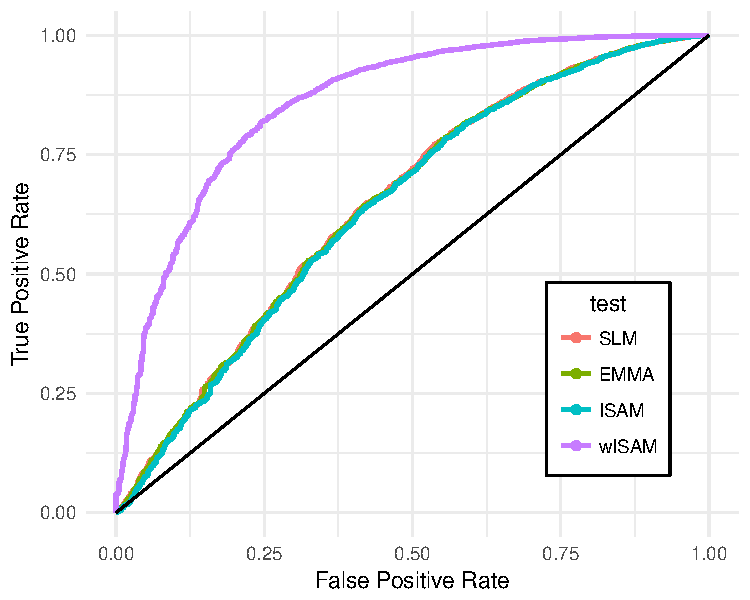
\includegraphics[width = 0.5\textwidth]{images/roc_hetsked_100snps_1ksims_05h2_100strains.pdf}
  \caption{explain this}
  \label{fig:exampleROC}
\end{figure}


\section{Software}